\documentclass[10pt, compress]{beamer}

\usetheme[usetotalslideindicator]{m}
\usepackage{booktabs}
\usepgfplotslibrary{dateplot}
\usepackage{listings}
\usepackage{amsmath,amssymb,nopageno}
\usepackage[all]{xy}
\usepackage{multirow}

\renewcommand{\today}{\ifnum\number\day<10 0\fi \number\day /%
\ifcase \month \or Janeiro\or Fevereiro\or Março\or Abril\or Maio%
\or Junho\or Julho\or Agosto\or Setembro\or Outubro\or Novembro\or Dezembro\fi /%
\number \year} 

\title{Introdução à Teoria Formal de Objetos}
\subtitle{}
\date{09 de Junho}
\author{Pedro Bruel, António Miranda}
\institute{Programação Orientada a Objetos 2015}

\begin{document}

\maketitle

\begin{frame}{Índice}
  \begin{columns}[onlytextwidth]
\column{0.5\textwidth}
      \begin{enumerate}
        \item Contextualização
            \begin{enumerate}
                \item Cálculo-$\lambda$
                \item Tipos e Categorias
                \item Exemplo
            \end{enumerate}
        \item Cálculo-$\varsigma$
            \begin{enumerate}
                \item Primitiva objeto
                \item Semântica das primitivas
                \item Sintaxe
                \item Exemplo da calculadora
                \item Classe
                \item Herança
            \end{enumerate}
      \end{enumerate}
  \end{columns}
\end{frame}

\section{Contextualização}

\begin{frame}[fragile]
  \frametitle{Cálculo-$\lambda$}
    \begin{itemize}
        \item É um sistema formal para expressão de cálculos;
        \item Representa a Aplicação e Abstração de funções;
        \item Pode ser Tipado ou Não-Tipado;
        \pause
        \item Aplicação ao "Problema de Decisão" (\emph{Entscheidungsproblem});
        \item Implementação de Linguagens Funcionais.
  \end{itemize}
\end{frame}

\begin{frame}[fragile]
  \frametitle{Cálculo-$\lambda$}
  \begin{figure}[H]
      \centering
      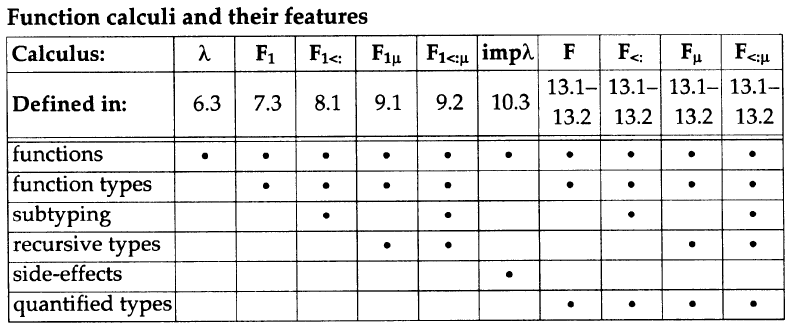
\includegraphics[width=1\textwidth]{functioncalculi.png}
  \end{figure}
\end{frame}

\begin{frame}[fragile]
  \frametitle{Cálculo-$\lambda$: Definição}
  \begin{block}{Expressões são compostas de:}
      \begin{itemize}
          \item $v_1, v_2, \ldots, v_n$
          \item Abstração: $\lambda$ e $.$
          \item Aplicação: $()$
      \end{itemize}
  \end{block}
  \pause
  \begin{block}{Conjunto $\Lambda$ de Expressões:}
      \begin{itemize}
          \item $x \in \Lambda$
          \item $x \in \Lambda, M \in \Lambda \Rightarrow ({\lambda}x.M) \in \Lambda$
          \item $M, N \in \Lambda \Rightarrow (M,N) \in \Lambda$
      \end{itemize}
  \end{block}
\end{frame}

\begin{frame}[fragile]
  \frametitle{Cálculo-$\lambda$: Definição}
  \begin{block}{Variáveis Livres:}
      \begin{itemize}
          \item $FV(x) = \{x\}$
          \item $FV({\lambda}x.M) = FV(M) \backslash \{x\}$
          \item $FV(M N) = FV(M) \bigcup FV(N)$
      \end{itemize}
  \end{block}
  \pause
  \begin{block}{Representação em Lisp, Haskel, \ldots:}
      \begin{lstlisting}[language=Python, basicstyle=\ttfamily,keywordstyle=\color{red}]
          (lambda (x) (* x x))
      \end{lstlisting}
  \end{block}
\end{frame}

\section{Tipos e Categorias}

\begin{frame}[fragile]
  \frametitle{Teoria de Tipos}
  \begin{block}{\emph{Principia Mathematica}:}
      \begin{itemize}
          \item Problema: Paradoxo de Russel;
          \pause
          \item Solução: Restringir operações a certos Tipos.
      \end{itemize}
  \end{block}
  \pause
  \begin{block}{Exemplo em julialang:}
      \begin{lstlisting}[language=Python, basicstyle=\ttfamily,keywordstyle=\color{red}]
(Integer       <: Number)        => true
(FloatingPoint <: Number)        => true
(Int64         <: Integer)       => true
(Float64       <: FloatingPoint) => true
(ASCIIString   <: Number)        => false
      \end{lstlisting}
  \end{block}
\end{frame}

\begin{frame}[fragile]
  \frametitle{Teoria de Categorias}
  \textbf{Categorias:}
  \begin{itemize}
      \item Estruturas compostas de \emph{objetos} e \emph{morfismos};
      \item Analogia com Sistemas de Tipos.
  \end{itemize}
  \pause
  \huge
  \begin{equation*}
      \xymatrix{
          A \ar@(l,u)^{1_A}[] \ar_{g \circ f}[dr] \ar^f[r] & B \ar@(u,r)^{1_B}[] \ar^g[d]\\
                                                           &C \ar@(d,r)_{1_C}[]
      }
  \end{equation*}
\end{frame}

\begin{frame}[fragile]
  \frametitle{Teoria de Categorias}
  \textbf{Sistema de Tipos como Categoria:}
  \begin{figure}[H]
      \centering
      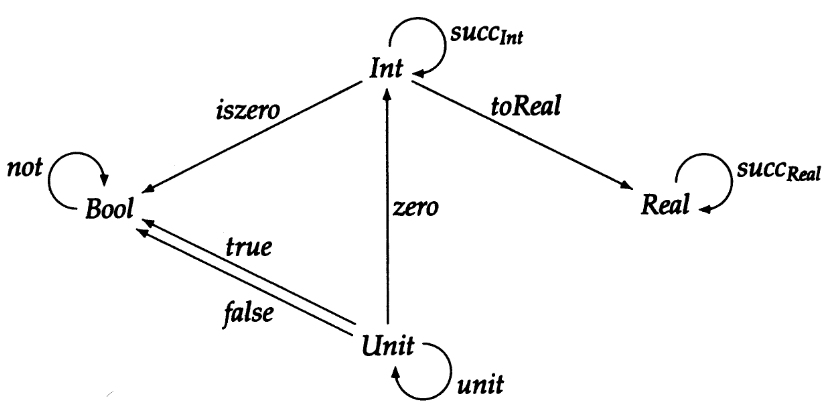
\includegraphics[width=0.8\textwidth]{categories_types.png}
  \end{figure}
\end{frame}

\begin{frame}[fragile]
  \frametitle{Exemplo}
  \begin{block}{Covariância e Contravariância:}
      \begin{itemize}
          \item Propriedades de \emph{Functores} (Mapeamentos entre Categorias);
          \item Contravariância: Mapeamento do oposto de uma Categoria.
      \end{itemize}
  \end{block}
  \pause
  \begin{block}{Em Linguagens Orientadas a Objetos:}
      \begin{itemize}
          \item Restrição de operações a certos tipos e subtipos;
          \item Relações entre tipos;
      \end{itemize}
  \end{block}
\end{frame}

\begin{frame}[fragile]
  \frametitle{Exemplo: Covariância}
  Sejam $A$ e $B$ tipos, então a composição $AxB$ 
  é covariante nos dois tipos, pois:
  
    $AxB <: A'xB' \Leftrightarrow A <: A', B <: B'$
  \pause
  \begin{block}{Exemplo em julialang:}
      \small
      \begin{lstlisting}[language=Python, basicstyle=\ttfamily,keywordstyle=\color{red}]
typeof((2::Int64, 2.0::Float64)) <: (Number, Number)
true
typeof((2::Int64, 2.0::Float64)) <: (Integer, FloatingPoint)
true
typeof((2::Int64, 2.0::Float64)) <: (Integer, Integer)
false
      \end{lstlisting}
  \end{block}
\end{frame}

\begin{frame}[fragile]
  \frametitle{Exemplo: Contravariância}
  Sejam $A$ e $B$ tipos, então a função $f: A \rightarrow B$
  é covariante em $B$, mas contravariante em $A$, pois: 
  
    $f: A \rightarrow B <: f: A' \rightarrow B' \Leftrightarrow A' <: A, B <: B'$
  \pause
  \begin{block}{Exemplo em julialang:}
      \small
      \begin{lstlisting}[language=Python, basicstyle=\ttfamily,keywordstyle=\color{red}]
function f{T <: Integer}(n::T)
   return string(n)
end
      \end{lstlisting}
  \end{block}
\end{frame}

\begin{frame}[fragile]
  \frametitle{Object Calculi}
  \begin{figure}[H]
      \centering
      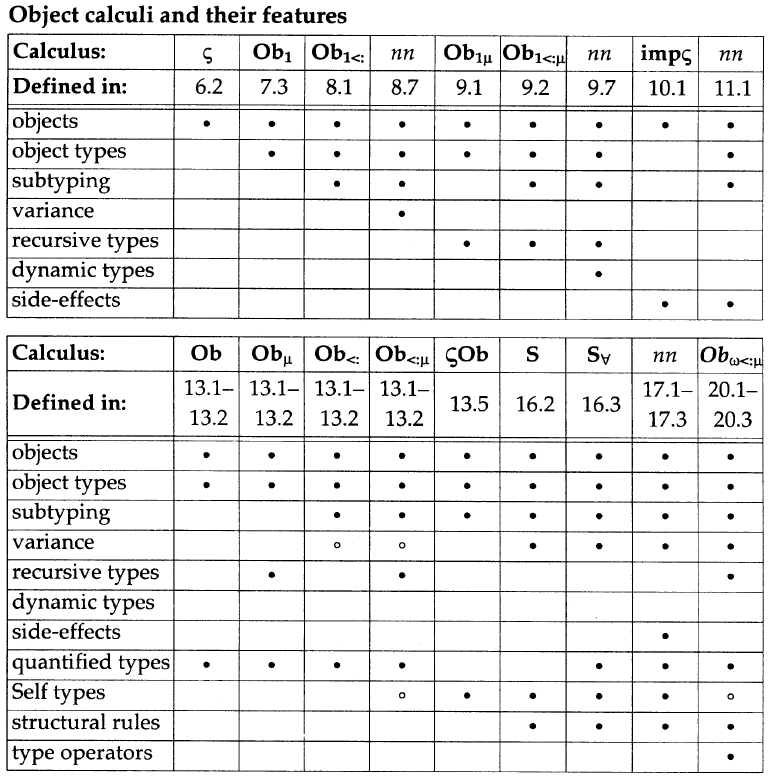
\includegraphics[width=0.6\textwidth]{objectcalculi.png}
  \end{figure}
\end{frame}

\section{Cálculo-$\varsigma$}

\begin{frame}[fragile]
  \frametitle{Cálculo-$\varsigma$}
  Para formalizar a ideia de um objeto, no livro \textit{A theory of objects} de Martín Abadi e Luca Cardelli,
  foi desenvolvido o cálculo-$\varsigma$ (sigma).
  \\~\\                                                                                                                                              
  Baseado no já conhecido cálculo-$\lambda$ (lambda), trata-se de um cálculo não-tipado que 
  define a semântica para os objetos e trata-os como primitivas.
\end{frame}

\begin{frame}[fragile]
  \frametitle{Cálculo-$\varsigma$: Primitiva Objeto}
  No cálculo-$\varsigma$, um objeto é considerado uma estrutura computacional.
  É uma coleção de atributos (não anônimos), onde todos são métodos.
  \\~\\
  Um método é composto por uma variável que representa o \textit{self} e por um corpo que produz o resultado.
  \\~\\
  As únicas operações válidas sobre objetos são atualização e invocação de métodos.
\end{frame}         

\begin{frame}[fragile]
  \frametitle{Cálculo-$\varsigma$: Primitiva Objeto}
  A notação usada para um objeto e seus métodos:
  \begin{itemize}
  \item $\varsigma$(x)b - método com x como parâmetro \textit{self} e corpo b;
  \item $[l_{1}$ = $\varsigma$($x_{1}$)$b_{1}$, $\ldots$, $l_{n}$=$\varsigma$($x_{n}$)$b_{n}]$ 
    - um objeto com n métodos, onde cada método é identificado pelo $l_{1}$, $\ldots$, $l_{n}$;
  \item o.l - o objeto o invoca o método l;
  \item o.l $^{\leftharpoonup}_{\leftharpoondown}$  $\varsigma$(x)b - atualizando o método l do 
    objeto o com o método $\varsigma$(x)b (a atualização de um método produz uma cópia do objeto 
    o com o $\varsigma$(x)b no lugar do método l).
  \end{itemize}
  Exemplo de um objeto:  [$l_{1}$=$\varsigma$($x_{1}$)[], $l_{2}$=$\varsigma$($x_{2}$)$x_{2}$.$l_{1}$]
\end{frame}

\begin{frame}[fragile]
  \frametitle{Cálculo-$\varsigma$: Primitiva Objeto}
  Métodos que não usam o parâmetro \textit{self}, $l_{1}=\varsigma(x_{1})[]$ do exemplo anterior, são considerados 
  campos do objeto. Simplificações na notação de um campo:
  \begin{itemize}
  \item $[\ldots, l=b, \ldots]$ é equivalente a $[\ldots, l=\varsigma(y)b, \ldots]$ para um parâmetro y (\textit{self}) 
    não usado (declaração de um campo);
  \item o.l := b é equivalente a o.l $^{\leftharpoonup}_{\leftharpoondown}$  $\varsigma$(y)b para um y não usado (atualização de um campo).
  \end{itemize}
  Terminologia para atributos e operações num objeto:
  \\~\\
  \begin{tabular}{cc|c|c|}
    \cline{3-4}
    & & \multicolumn{2}{ c| }{Atributos} \\ \cline{3-4}
    & & campos & métodos \\ \cline{1-4}
    \multicolumn{1}{ |c  }{\multirow{2}{*}{Operações} } &
    \multicolumn{1}{ |c| }{seleção} & seleção & invocação \\ \cline{2-4}
    \multicolumn{1}{ |c  }{}                        &
    \multicolumn{1}{ |c| }{atualização} & atualização & atualização \\ \cline{1-4}
  \end{tabular}
\end{frame}

\begin{frame}[fragile]
  \frametitle{Cálculo-$\varsigma$: Semântica das primitivas}
  A execução de um termo num cálculo-$\varsigma$ pode ser expresso como uma sequência de redução de passos.
  Isso é conhecido por {\bf semântica primitiva}. Ela representa da forma mais simples e direta possível a
  semântica pretendida do objeto.
  \\~\\
  Para definir essas semânticas primitivas, foram introduzidas as seguintes notações:
  \begin{itemize}
  \item $\Phi_{i}$ $^{i \in 1 \ldots n}$ denota $\Phi_{1}$, $\Phi_{2}$, $\ldots$, $\Phi_{n}$;
  \item b $\mapsto$ c significa que  b reduz a c em um passo;
  \item b \{\{x $\leftarrow$ c\}\} indica a substituição do termo c para as ocorrências de x em b.
  \end{itemize}
\end{frame}

\begin{frame}[fragile]
  \frametitle{Cálculo-$\varsigma$: Semântica das primitivas}
  Passos da redução para as operações existentes no cálculo-$\varsigma$:
  \\
  Seja o $\equiv$ [$l_{i}$ = $\varsigma$($x_{i}$)$b_{i}$ $^{i \in 1 \ldots n}$] um objeto, onde todos os $l_{i}$ são distintos. 
  \\
  Temos,
  \begin{itemize}
  \item o.$l_{j}$ $\mapsto$ $b_{j}$ \{\{$x_{j}$ $\leftarrow$ o\}\} (j $\in$ 1 $\ldots$ n) - redução de uma invocação;
  \item o.l $^{\leftharpoonup}_{\leftharpoondown}$ $\varsigma$(y)b $\mapsto$
    [$l_{j}$ = $\varsigma$(y)b, $l_{i}$ = $\varsigma$($x_{i}$)$b_{i}$ $^{i \in 1 \ldots n}$] (j $\in$ 1 $\ldots$ n) - redução de uma atualização.
  \end{itemize}
  A invocação do o.$l_{j}$ consiste na substituição do objeto \textit{host} pelo \textit{self} no copro do método $l_{j}$.
  \\
  A atualização do método o.l $^{\leftharpoonup}_{\leftharpoondown}$  $\varsigma$(y)b se reduz a uma cópia do objeto \textit{host}
  com o método trocado pela versão atualizada.
\end{frame}

\begin{frame}[fragile]
  \frametitle{Cálculo-$\varsigma$: Semântica das primitivas}
  Supondo que os símbolos $\dot{=}$ e $\equiv$  significam respectivamente ``igual por definição'' e ``sintaticamente igual'',
  vamos apontar alguns exemplos de reduções.
  \\~\\
  A substituição própria (\textit{self-substitution}) está no \textit{core} das semânticas primitivas da invocação de um método, 
  portanto, é fácil programar computações não-terminais sem o uso explícito da recursão.
  \\~\\
  Seja
  \\ 
  $o_{2}$ $\dot{=}$ [l = $\varsigma$(x)x.l]
  \\
  então 
  \\
  $o_{2}$.l $\mapsto$ x.l\{\{x $\leftarrow$ $o_{2}$\}\} $\equiv$ $o_{2}$.l $\mapsto$ $\ldots$
\end{frame}

\begin{frame}[fragile]
  \frametitle{Cálculo-$\varsigma$: Semântica das primitivas}
  A substituição própria também permite retornar e modificar o \textit{self}.
  \\~\\
  Seja
  \\
  $o_{3}$ $\dot{=}$ [l = $\varsigma$(x)x]
  \\
  então
  \\
  $o_{3}$.l $\mapsto$ x\{\{x $\leftarrow$ $o_{3}$\}\} $\equiv$ $o_{3}$
  \\~\\
  Seja
  \\
  $o_{4}$ $\dot{=}$ [l = $\varsigma$(y)(y.l $^{\leftharpoonup}_{\leftharpoondown}$ $\varsigma$(x)x)]
  \\
  então
  \\
  $o_{4}$.l $\mapsto$ (y.l  $^{\leftharpoonup}_{\leftharpoondown}$  $\varsigma$(x)x)\{\{y $\leftarrow$ $o_{4}$\}\} $\equiv$ $o_{3}$
  \\~\\
  OBS: Em linguagens baseadas em classes, é comum um método modificar seus atributos, apesar desses atributos serem campos e não
  métodos.
\end{frame}

\begin{frame}[fragile]
  \frametitle{Cálculo-$\varsigma$: Sintaxe}
  A sintaxe do cálculo-$\varsigma$ é descrita pela gramática baixo:
  \\~\\
  a,b ::= (termo)
  \\
  \hspace{1cm} x  (variável)
  \\
  \hspace{1cm} [$l_{i}$ = $\varsigma$($x_{i}$)$b_{i}$ (i $\in$ 1 $\ldots$ n)]  (criação de um objeto, $l_{i}$ distintos)
  \\
  \hspace{1cm} a.l  (seleção de campos ou invocação de métodos)
  \\
  \hspace{1cm} a.l $^{\leftharpoonup}_{\leftharpoondown}$  $\varsigma$(x)b  (atualização de campos ou métodos)
  \\~\\
  Qualquer expressão gerada por essa gramática é um termo-$\varsigma$.
  \\~\\
  A notação a,b ::= $\ldots$ descreve indutivamente um conjunto de expressões, onde a e b pertencem ao conjunto das expressões a
  serem definidos.
\end{frame}

\begin{frame}[fragile]
  \frametitle{Cálculo-$\varsigma$: Sintaxe}
  As outras definições significam que um termo a ou b podem ser uma:
  \begin{itemize}
  \item variável x;
  \item expressão da forma [$l_{i}$ = $\varsigma$($x_{i}$)$b_{i}$ $^{i \in 1 \ldots n}$] 
    (onde $l_{i}$ é um rótulo, $x_{i}$ é uma variável e $b_{i}$ é um termo);
  \item expressão da forma a.l (onde a é um termo e l é o rótulo de um método ou campo);
  \item expressão da forma a.l $^{\leftharpoonup}_{\leftharpoondown}$  $\varsigma$(x)b 
    (onde a e b são termos, l é o rótulo de um método ou campo e x uma variável).
  \end{itemize}
\end{frame}

\begin{frame}[fragile]
  \frametitle{Cálculo-$\varsigma$: Exemplo da calculadora}
  calculadora $\dot{=}$
  \\
  \hspace{0.5cm}[\hspace{0.5cm}arg = 0.0,
  \\
  \hspace{1cm} aux = 0.0,
  \\
  \hspace{1cm} inserir = $\varsigma$(s)$\lambda$(n)s.arg := n,
  \\
  \hspace{1cm} mais = $\varsigma$(s)(s.aux := s.igual).igual $^{\leftharpoonup}_{\leftharpoondown}$ $\varsigma$($s^{'}$)$s^{'}$.aux + $s^{'}$.arg,
  \\
  \hspace{1cm} menos = $\varsigma$(s)(s.aux := s.igual).igual $^{\leftharpoonup}_{\leftharpoondown}$ $\varsigma$($s^{'}$)$s^{'}$.aux - $s^{'}$.arg,
  \\
  \hspace{1cm} igual = $\varsigma$(s)s.arg,
  \\
  \hspace{1cm} reiniciar = $\varsigma$(s)(s.arg := 0.0).aux := 0.0 ]
  \\~\\
  As variáveis arg e aux são usadas nas operações internas da calculadora.
  \\
  Os métodos inserir, mais, menos, igual e reiniciar provêm a interface.
\end{frame}

\begin{frame}[fragile]
  \frametitle{Cálculo-$\varsigma$: Exemplo da calculadora}
  Exemplo de uso e comportamento da calculadora.
  \\~\\
  calculadora.inserir(5.0).igual = 5.0
  \\
  calculadora.inserir(5.0).menos.inserir(3.5).igual = 1.5
  \\
  calculadora.inserir(5.0).mais.mais.igual = 15.0
  \\
  calculadora.inserir(5.0).reiniciar = 0.0
\end{frame}

\begin{frame}[fragile]
  \frametitle{Cálculo-$\varsigma$: Classe}
  No cálculo-$\varsigma$, uma classe é considera um gerador de objetos com informações sobre si mesma.
  Em outras palavras podemos dizer que uma classe é uma coleção de pré-métodos (informações) que possui um
  método \textit{new} para gerar os novos objetos.
  \\~\\
  Um pré-método é um método da forma:
  \\
  \hspace{1cm} $l_{i}$ = $\varsigma$(z) $\lambda$($x_{i}$)$b_{i}$ onde i $\in$ 1 $\ldots$ n
  \\
  ou
  \\
  \hspace{1cm} $l_{i}$ = $\lambda$($x_{i}$)$b_{i}$ onde i $\in$ 1 $\ldots$ n
  \\~\\
  OBS:  Informações de uma classe (pré-métodos) podem ser contribuições de outras classes.
\end{frame}

\begin{frame}[fragile]
  \frametitle{Cálculo-$\varsigma$: Classe}
  c $\dot{=}$
  \\
  \hspace{0.5cm}[\hspace{0.5cm}new = $\varsigma$(z)[$l_{i}$ = $\varsigma$(s)z.$l_{i}$(s)$^{i \in 1 \ldots n}$],
  \\
  \hspace{1cm} $l_{i}$ = $\lambda$(s)$b_{i}$ $^{i \in 1 \ldots n}$ ]
  \\~\\
  O método \textit{new} simplesmente aplica o \textit{self} do novo objeto na coleção de pré-métodos da classe, que por
  conseguinte os transforma em métodos.
  \\
  Dada uma classe c, a invocação c.new um objeto do tipo c. Exemplo:
  \\
  \hspace{1cm} o $\dot{=}$ c.new = [$l_{i}$ = $\varsigma$($x_{i}$)$b_{i}$ $^{i \in 1 \ldots n}$]
\end{frame}

\begin{frame}[fragile]
  \frametitle{Cálculo-$\varsigma$: Herança}
  Consiste em reusar pré-métodos entre classes (ou \textit{traits}). Exemplo, se uma classe $c^{'}$ é definida reusando todos os pré-métodos
  de uma classe c (c.$l_{j}$ $j \in 1 \ldots n$) e adicionando mais pré-métodos ($\lambda$(s)$b_{k}$ $^{k \in n+1 \ldots n+m}$),
  informalmente podemos dizer que $c^{'}$ é uma subclasse de c.
  \\~\\
  $c^{'}$ $\dot{=}$
  \\
  \hspace{0.5cm}[\hspace{0.5cm}new = $\varsigma$(z)[$l_{i}$ = $\varsigma$(s)z.$l_{i}$(s)$^{i \in 1 \ldots n+m}$],
  \\
  \hspace{1cm} $l_{j}$ = c.$l_{j}$ $^{j \in 1 \ldots n}$,
  \\
  \hspace{1cm} $l_{k}$ = $\lambda$(s)$b_{k}$ $^{k \in n+1 \ldots n+m}$ ]
\end{frame}

\begin{frame}[fragile]
  \frametitle{Cálculo-$\varsigma$: Herança}
  Uma subclasse pode sobrescrever pré-métodos em vez de herdá-los. Exemplo, se uma classe $c^{''}$ é definida reusando os primeiros
  n-1 pré-métodos de uma classe c e sobrecarregando o último pré-método.
  \\~\\
  $c^{''}$ $\dot{=}$
  \\
  \hspace{0.5cm}[\hspace{0.5cm}new = $\varsigma$(z)[$l_{i}$ = $\varsigma$(s)z.$l_{i}$(s)$^{i \in 1 \ldots n}$],
  \\
  \hspace{1cm} $l_{j}$ = c.$l_{j}$ $^{j \in 1 \ldots n-1}$,
  \\
  \hspace{1cm} $l_{k}$ = $\lambda$(s) $\ldots$ c.$l_{n}$(s) $\ldots$ c.$l_{p}$(s) $\ldots$ ]
  \\~\\
  O método sobrecarregado $l_{n}$ pode referenciar a um pré-método original de c como c.$l_{n}$, ou até a um outro pré-método de uma
  super classe de c, com c.$l_{p}$, onde p $\in 1 \ldots n$. Assim modelamos o comportamento do {\bf super}.
  \\
  OBS: A herança múltipla é obtida através do reúso de pré-métodos de múltiplas classes (ou \textit{traits}).
\end{frame}

\section{Referências}

\begin{frame}[fragile]
  \frametitle{Referências}
  \begin{enumerate}
  \item Abadi, M., e Cardelli, L. (1996). {\textit A theory of objects}. Springer Science \& Business Media.
  %\item Bruce, K.(2002). {\textit Foundations of Object-Oriented Languages types and semantics}. The MIT Press.
  \item Pierce, B. (2002). {\textit Types and programming Languages}. The MIT Press.
  \end{enumerate}
\end{frame}

\plain{Obrigado! Perguntas?}

\end{document}
